% -*- LaTeX -*-
% -*- coding: utf-8 -*-
%
% michael a.g. aïvázis
% california institute of technology
% (c) 1998-2012 all rights reserved
%

\documentclass[12pt,answers]{exam}

% packages, setup, macros, etc.
% -*- LaTeX -*-
% -*- coding: utf-8 -*-
%
% ~~~~~~~~~~~~~~~~~~~~~~~~~~~~~~~~~~~~~~~~~~~~~~~~~~~~~~~~~~~~~~~~~~~~~~~~~~~~~~
%
%                             michael a.g. aïvázis
%                      california institute of technology
%                      (c) 1998-2010  all rights reserved
%
% ~~~~~~~~~~~~~~~~~~~~~~~~~~~~~~~~~~~~~~~~~~~~~~~~~~~~~~~~~~~~~~~~~~~~~~~~~~~~~~
%


% language
\usepackage[english]{babel}

% color
\usepackage{xcolor}

% fonts
\usepackage{amsfonts}
\usepackage{times}
%\usepackage[iso-8859-7]{inputenc}

% figures
\usepackage{graphicx}

% listings and their configurations
\usepackage[slide,algoruled,linesnumbered,noend]{algorithm2e}
\SetKwComment{tnm}{\#}{}
\SetKw{KwAnd}{and}
\SetKw{KwSend}{send}
\SetKw{KwRecv}{recv}
\SetKw{KwFrom}{from}

\usepackage{textcomp}
\usepackage{listings}
\definecolor{keywordcolor}{rgb}{.0,.0,1.0}
\definecolor{commentcolor}{gray}{.3}
\definecolor{stringcolor}{gray}{.0}
\definecolor{linenumbercolor}{gray}{.3}
\definecolor{listingbgcolor}{gray}{.97}

\definecolor{acm114@sand}{HTML}{dddbc5}
\definecolor{acm114@olive}{HTML}{474a41}
\definecolor{acm114@lava}{HTML}{413b38}

\lstnewenvironment{python}[2][]{
  \lstset{
    language=python,
    morekeywords={self,yield,False,True,None},
    %
    columns=flexible,
    upquote=true,
    %
    aboveskip=\bigskipamount,
    belowskip=\bigskipamount,
    %
    numbers=left,
    numberstyle=\color{linenumbercolor}\tiny,
    stepnumber=1,
    numbersep=5pt,
    numberblanklines=true,
    %
    basicstyle=\tt\scriptsize,
    keywordstyle=\color{keywordcolor},
    commentstyle=\color{commentcolor}\slshape,
    stringstyle=\color{stringcolor}\slshape,
    showstringspaces=false,
    %
    frame=tb,
    captionpos=t,
    backgroundcolor=\color{white},
    xleftmargin=.25in,
    xrightmargin=.1in,
    %
    escapeinside={\#@}{@},
    %
    #1
  }}{#2}

\lstnewenvironment{C}[1][]{
  \lstset{
    language=c,
    columns=flexible,
    upquote=true,
    %
    aboveskip=\bigskipamount,
    belowskip=\bigskipamount,
    %
    numbers=left,
    numberstyle=\color{linenumbercolor}\tiny,
    stepnumber=1,
    numbersep=5pt,
    numberblanklines=true,
    %
    basicstyle=\tt\scriptsize,
    keywordstyle=\color{blue},
    commentstyle=\color{commentcolor}\slshape,
    showstringspaces=false,
    %
    frame=tb,
    captionpos=t,
    backgroundcolor=\color{listingbgcolor},
    xleftmargin=.25in,
    xrightmargin=.1in,
    %
    escapeinside={//@}{@},
    %
    #1
  }}{}

% references
\usepackage[numbers]{natbib}
\bibliographystyle{unsrtnat}
\renewcommand\bibsection{\section{\refname}}
\def\newblock{\small}

% misc
\usepackage{dcolumn}
\newcolumntype{d}[1]{D{.}{.}{#1}}

\usepackage{url}
\usepackage{hyperref}


% shortcuts
\def\algref#1{{Alg.~\ref{alg:#1}}}
\def\alglineref#1{{line~\ref{line:#1}}}
\def\eqref#1{{Eq.~\ref{eq:#1}}}
\def\figref#1{{Fig.~\ref{fig:#1}}}
\def\secref#1{{Sec.~\ref{sec:#1}}}
\def\tabref#1{{Table~\ref{tab:#1}}}
\def\lstref#1{{Listing~\ref{lst:#1}}}
\def\lstlineref#1{{line~\ref{line:#1}}}

% macros
\def\bydef{\mathrel{\mathop:}=}
\def\CC{\mbox{\tt C}}
\def\GNU{\mbox{\tt GNU}}
\def\GSL{\mbox{\tt GSL}}
\def\RANLUX{\mbox{\tt RANLUX}}

\def\cpp{\mbox{\tt C++}}
%\def\cpp{\mbox{\tt C\raise.4ex\hbox{++}}}
\def\fortran{{\tt FORTRAN}}
\def\f90{{\tt FORTRAN90}}

\def\pyre{{\tt pyre}}

\def\order#1{\mbox{$\mathcal{O}(#1)$}}
\def\class#1{\mbox{\tt #1}}
\def\component#1{\mbox{\tt #1}}
\def\function#1{\mbox{\tt #1}}
\def\method#1{\mbox{\tt #1}}
\def\identifier#1{\mbox{\tt #1}}
\def\keyword#1{\mbox{\tt #1}}
\def\srcfile#1{\mbox{\tt #1}}

\def\insertionsort{\mbox{\sc Insertion-Sort}}
\def\mergesort{\mbox{\sc Merge-Sort}}
\def\merge{\mbox{\sc Merge}}

\def\TODO#1{{%
\subsubsection*{Still to do}%
\scriptsize\tt%
\begin{list}{\leftpointright}{} #1 \end{list}}}

% set up the PDF options
\hypersetup{
    pdftitle={ACM/CS 114: Winter 2010},
    pdfauthor={Michael A.G. A\"iv\'azis},
    pdfsubject={Lecture notes},
    pdfkeywords=,           % list of keywords
%
    bookmarks=true,         % show bookmarks bar?
    unicode=false,          % non-Latin characters in Acrobat's bookmarks
    pdftoolbar=true,        % show Acrobat's toolbar?
    pdfmenubar=true,        % show Acrobat's menu?
    pdffitwindow=true,      % page fit to window when opened
    pdfnewwindow=true,      % links in new window
    colorlinks=true,        % false: boxed links; true: colored links
    linkcolor=acm114@sand,  % color of internal links
    citecolor=acm114@sand,  % color of links to bibliography
    filecolor=acm114@sand,  % color of file links
    urlcolor=acm114@sand    % color of external links
}
% end of file 


\begin{document}
\pagestyle{headandfoot}
\runningfootrule
\firstpageheader{ACM/CS 114}{Assignment 3}{Due: 15 Feb 2012}
\runningheader{}{}{}
\firstpagefooter{}{}{}
\runningfooter{ACM/CS 114}{Assignment 2}{\thepage}


% --------------------------------------
% Monte Carlo integration
\def\Li{\mbox{\rm Li}_{2}}
\def\dilog{\mbox{\tt dilog}}

In this assignment, we will use Monte Carlo integration to compute an approximation to the
value of $\pi$ by computing the area of the upper right quadrant of a unit circle centered at
the origin, as shown in \figref{pie}.
%
\begin{figure}[h]
\centering
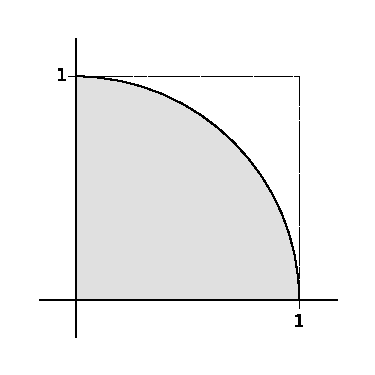
\includegraphics[scale=.75]{pie.pdf}
\caption{Estimating $\pi$ by computing the area of a quadrant of the unit circle
  \label{fig:pie}}
\end{figure}
%

You can get an estimate for $\pi/4$ by generating random points in the unit box and counting
the fraction that fall within the shaded quarter circle.


\begin{questions}

\question The effectiveness of computing using stochastic techniques is intimately related to
the properties of the pseudo-random generator used.

\begin{parts}
  \part Choose a random number generator and use it to fill a container with 10 numbers between
  0 and 1. Do you get the same 10 numbers every time you run the program? How can you seed your
  generator so that each execution of your program produces the same sequence? How can you seed
  it so that each execution produces different random numbers?

  \part Use your generator to fill a container with $10^6$ numbers between 0 and 1. Partition
  the interval $[0,1]$ into 10 bins of equal width and build a frequency histogram, i.e.~plot
  the number of times random numbers from your container fall within each bin. What is the
  average occupancy of the bins? What is the standard deviation?

  \part Repeat the above steps using 100 bins.

\end{parts}

\question Compute the Monte Carlo estimate for $\pi$ from \figref{pie}.

\begin{parts}

\part Implement the sequential version. How many points are required to get the error to
drop below $10^{-3}$. Below $10^{-5}$?

\part Implement a parallel version using threads. Make sure that your random number
generator is thread safe.

\part Implement a parallel version using \mpi. Make sure that you seed your generator properly
so that each process gets a different sequence of random numbers.
\end{parts}

\question Monte Carlo integration converges to the answer very slowly. However, it has the
great advantage that its convergence properties are not affected by the dimensionality of the
problem. Adapt one of your parallel implementations to compute another estimate for $\pi$ using
the volume of the positive octant of a unit ball centered at the origin. How many points in
three dimensions does it take to get the error to  drop below $10^{-5}$?

\end{questions}

\end{document}

% end of file 
